\chapter{Návrh modelu}\label{chap:proposal}

V tejto kapitole sa budem venovať návrhu samotného modelu a pokúsim sa takisto objasniť dôvody, ktoré ma viedli ku konkrétnym rozhodnutiam. Návrh nášho modelu, ktorý je súčasťou tejto diplomovej práce je inšpirovaný dvoma existujúcim modelmi, konkrétne náš model je podobne ako model od Busaryev a spol. \cite{busaryev2012} založený na princípe pružinového systému a na výpočet rýchlostí bublín v čase $t + 1$ využívame implicitnú metódu taktiež z tohto článku, ktorá bola pôvodne použitá v článku od Choi a Ko \cite{choiko2002}, kde bola táto metóda využitá pri simulácii látok. Z článku od Sunkel a spol. \cite{sunkel2004} zase náš model využíva myšlienku posúvania vrcholov dvoch dotýkajúcich sa bublín na ich spoločnú stenu. Simulácia aj vizualizácia nášho modelu bude prebiehať v 3D.

\section{Pružinový systém}

Pružinový systém, niekedy nazývaný tiež pružinová sieť, je fyzikálny model, popísaný ako graf, kde každý vrchol má svoju pozíciu a pozdĺž každej hrany tohto grafu je pružina s definovanou tvrdosťou. Za predpokladu, že sú tieto tieto pružiny lineárne a dochádza len k malým deformáciam, môže byť tento pružinový systém redukovaný na systém lineárnych rovníc, resp. problém minimalizácie energie. Existuje viacero typov pružinových systémov. Náš model využíva konkrétne pružinový systém s masou. V prípade, že je pružina natiahnutá, alebo stlačená pôsobením masy, vyprodukuje táto pružina tzv. obnovovaciu silu na získanie jej pôvodnej pokojovej dĺžky $L$. Hookove pravidlá popisujú vzťah tejto sily vyvíjanej pružinou, keď je natiahnutá alebo stlačená na konkrétnu dĺžku.

\begin{equation}
	F_{rest} \left( t \right) = -kx \left( t \right),
\end{equation}
kde $F_{rest}$ je obnovovacia sila, $k$ je konštanta tvrdosti pružiny a $x$ je posunutie masy vzhľadom na pozíciu v rovnovážnom stave. Znamienko mínus v tejto rovnici indikuje, že táto sila vyvíjaná pružinou vždy smeruje v opačnom smere vzhľadom na posunutie, inak povedané, táto sila vždy pôsobí smerom k nulovej (pokojovej) pozícii a tým zabraňuje mase k posúvaniu sa do nekonečna.

\section{Reprezentácia peny}

Geometrická štruktúra peny je veľmi komplexná, nakoľko je tvorená množstvom bublín, ktoré na seba vplývajú a deformujú sa, čím vytvárajú rôzne nepravidelné tvary. Jedným z cieľov tejto diplomovej práce je simulácia a vizualizácia peny v reálnom čase, preto každé zjednodušenie, ktoré nám ušetrí výpočtový čas a zároveň sa zásadným spôsobom neodkloní od vzhľadu a správania sa peny v reálnom svete, je pre náš model veľmi cenné. 

V reálnom svete majú bubliny nepravidelný tvar zapríčinený pôsobením rôznych síl na bublinu. Avšak čím je bublina menšia, tým skôr dokáže nadobudnúť späť svoj pôvodný guľovitý tvar. Keďže pena väčšinou obsahuje malé alebo stredne veľké bubliny, ktoré sú menej náchylné na deformácie, rozhodli sme sa naše bubliny aproximovať na tvar gule, čo nám ušetrí veľa výpočtového času, keďže nemusíme riešiť rôzne nepravidelné deformácie jednotlivých bublín peny.

Spoločná stena medzi bublinami je zakrivená vždy smerom do väčšej bubliny, čo je spôsobené väčším vnútorným tlakom v menšej bubline. Keďže počítanie tohto zakrivenia by takisto zvýšilo výpočtový čas, rozhodli sme sa spoločné steny bublín aproximovať na roviny.

\section{Sily pôsobiace na bubliny peny}

\begin{minipage}{\textwidth}
	Sily v našom modeli možno rozdeliť do dvoch skupín:
	\begin{itemize}
		\item interné sily
		\item externé sily
	\end{itemize}
\end{minipage}\newline

Medzi \textit{interné sily} patria sily pôsobiace vrámci peny, konkrétne ide o sily pôsobiace medzi bublinami. Sú to konkrétne dve sily: príťažlivá sila a odpudivá sila. Obidve tieto sily pôsobia medzi každými dvoma bublinami v modeli, ktorých vzdialenosť je menšia ako súčet ich polomerov, t.j. medzi bublinami, ktoré sa dotýkajú. Keďže náš model využíva pružinový systém, tieto sily v našom modeli simuluje iba jedna sila, a to konkrétne \textit{pružinová sila}.

Uvažujme dve bubliny $B_{i} = (p_{i}, r_{i}), B_{j} = (p_{j}, r_{j})$ v tomto systéme ( $p_{i}$ je pozícia (stred) a $r_{i}$ je polomer bubliny $B_{i}$ ), ktoré sa dotýkajú a sú teda spojené pružinou. 

\begin{figure}[H]
	\begin{center}
		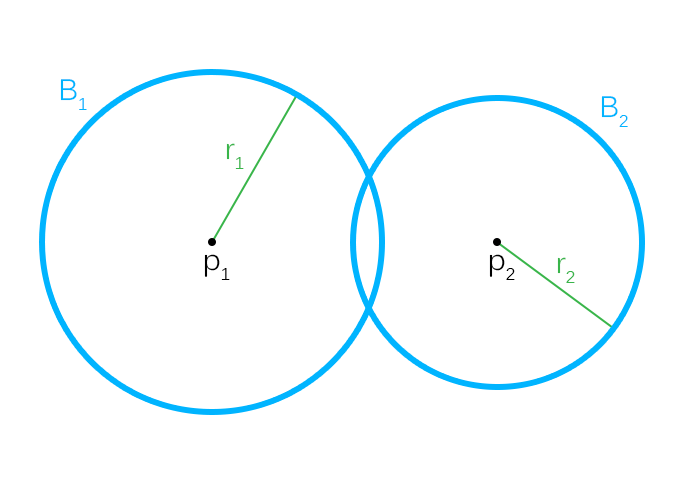
\includegraphics[height=\imageHeight]{images/bubbles_legend}
		\caption{Bubliny a ich pojmy.}
		\label{img:verticies_displacement_2}
	\end{center}
\end{figure}

\noindent
Nech $L_{ij}$ je pokojová dĺžka tejto pružiny. Táto dĺžka vyjadruje optimálnu a požadovanú vzdialenosť dvoch bublín odvodenú z Plateauových zákonov a vypočítame ju nasledovne:
\begin{equation}
	L_{ij}^{2} = r_{i}^{2} + r_{j}^{2} - r_{i}r_{j}.
\end{equation} 
Energiu pôsobiacu medzi týmito dvoma bublinami môžeme potom zapísať takto:
\begin{equation}
	\label{eq:spring_system_energy}
	E = \frac{1}{2}k_{s}\left ( \left | p_{ij} \right | - L_{ij} \right )^{2},
\end{equation} 
kde $p_{ij} = p_{j} - p_{i}$, a $k_{s}$ je konštanta tvrdosti pružiny. Z rovnice \reference{eq:spring_system_energy} vidno, že táto energia je rovná nule v prípade, že platí rovnosť $p_{ij} = L_{ij}$. Sila pôsobiaca na bublinu $B_{i}$ vzhľadom na deformáciu medzi týmito dvomi bublinami môžeme potom vyjadriť nasledovne:
\begin{equation}
	\label{eq:spring_system_force_on_bubble}
	f_{ij}^{spring} = -\frac{\partial E}{\partial p_{i}} = -k_{s}\left ( \left | p_{ij} \right | - L_{ij} \right )\frac{p_{ij}}{\left | p_{ij} \right |}.
\end{equation} 
Celková sila pôsobiaca na bublinu $B_{i}$ vyzerá nasledovne:
\begin{equation}
	\label{eq:spring_system_total_int_force}
	f_{i}^{int} = \sum_{j\; \in \; O_{i}}\left ( f_{ij}^{spring} \right ),
\end{equation}
kde $O_{i}$ je okolie bubliny $B_{i}$ pod ktorým rozumieme $\forall B_{j}$, ktoré sa dotýkajú s bublinou $B_{i}$.

Pri týchto silách môže dôjsť k oscilovaniu jednotlivých pružín medzi bublinami, čo je veľmi nežiadúci efekt v prípade peny a priťahovania sa bublín navzájom. Aby sme zabránili oscilácii pružín, obsahuje náš model ešte jednu internú silu, a to konkrétne \textit{tlmiacu silu}, ktorá má na starosti potlačiť tento efekt a jej rovnica vyzerá nasledovne:
\begin{equation}
	\label{eq:spring_system_damping_force}
	f^{damp} = -c_{vis}v - c_{lap}Lv,
\end{equation}
kde $c_{vis}, c_{lap}$ sú tlmiace koeficienty, $v$ je vektor rýchlostí bublín a $L$ je normalizovaná Laplaceova matica.

\subsubsection{Laplaceova matica}

Laplaceova matica neorientovaného acyklického grafu $G = (V, E)$, kde $n = \left | V \right |$, je symetrická matica veľkosti $n \times n$ definovaná ako:
\begin{equation}
	\label{eq:laplacian_matrix}
	L = D - A,
\end{equation}
kde $D = diag(d_{1}, ..., d_{n})$ je diagonálna matica stupňov vrcholov a $A$ je matica susedností. Diagonálne elementy $l{ij}$ matice $L$ zodpovedajú stupňu vrchola $v_{i}$ a mimodiagonálne elementy $l_{ij}$ sa rovnajú $-1$, ak vrchol $v_{i}$ je susedný k vrcholu $v_{j}$, resp. $0$ naopak. Laplaceova matica sa využíva na účely merania do akej miery sa graf líši v konkrétnom vrchole od okolitých vrcholov. \newline
Normalizovaná Laplaceova matica je definovaná takto:
\begin{equation}
	\label{eq:normalized_laplacian_matrix}
	L_{ij}(G) = \left\{\begin{matrix}
	1, & \textrm{ak }i = j\textrm{ a }d_{j} \neq 0\\ 
	-\frac{1}{\sqrt{d_{i}d_{j}}}, & \textrm{ak } i \textrm{ a } j \textrm{ susedia}\\ 
	0, & \textrm{inak}
	\end{matrix}\right.
\end{equation}

Pri \textit{externých silách} sme sa rozhodli použiť nakoniec len gravitačnú silu $f^{grav} = m_{i}g$, kde $m_{i}$ je hmotnosť bubliny $B_{i}$ a $g = 9.78 m/s^{2}$ je gravitačné zrýchlenie.

\section{Simulácia}

Na simuláciu peny využívame implicitnú metódu, ktorá je prezentovaná v článku od Busaryev a spol. \cite{busaryev2012} a ktorú pôvodne navrhli Choi a Ko \cite{choiko2002} v ich článku o simulácii látok.

\subsection*{Systém lineárnych rovníc}

Implicitná metóda, ktorú používame v našom modeli, rieši systém lineárnych rovníc s využitím spätnej Eulerovej metódy. Systém lineárnych rovníc je množina $k$ lineárnych rovníc s $n$ premennými. Vyriešením tejto sústavy dostávame $n$ hodnôt, ktoré sú riešením tohto systému, to znamená, že každá z rovníc je splnená. Jednoduchý systém lineárnych rovníc vyzerá nasledovne:\begin{equation}
\begin{split}
	a_{11}x_{1} + a_{12}x_{2} = b_{1}, \\
	a_{21}x_{1} + a_{22}x_{2} = b_{2},
\end{split}
\end{equation}
kde $x_{1}, x_{2}$ sú neznáme tohoto systému, $a_{11}, a_{12}, a_{21}, a_{22}$ sú koeficienty a $b_{1}, b_{2}$ sú konštanty. Najjednoduchšia metóda riešenia systému lineárnych rovníc je opakované odstraňovanie premenných. Táto metóda funguje nasledovne:
\begin{enumerate}
	\item Prvú rovnicu vyriešime pre jednu premennú.
	\item Následne túto premennú dosadíme do zvyšných rovníc.
	\item Pokračujeme dokiaľ nedostaneme jednu lineárnu rovnicu.
	\item Následne vyriešime túto lineárnu rovnicu a spätným dosádzaním do rovníc dostávame celkové riešenie tohto systému.
\end{enumerate} 

Systém lineárnych rovníc sa dá tiež zapísať v maticovom tvare $Ax = b$, kde $A$ je tzv. matica systému, ktorá obsahuje koeficienty rovníc. Matica, alebo skôr vektor $b$ obsahuje pravé strany rovníc tohto systému a vektor $x$ obsahuje premenné tohto systému. V prípade, že tento systém obsahuje veľké množstvo rovníc, určiť presné riešenie takéhoto systému môže byť výpočtovo veľmi náročné. Preto sa v takomto prípade zvyknú na výpočet použiť tzv. iteratívne metódy, ktoré hľadajú približné riešenie konvergujúce k správnemu riešeniu. Iteratívna metóda, ktorú používame v našom modeli sa nazýva metóda združených gradientov, pri ktorej musí platiť, že matica systému $A$ je symetrická.

\newpage

Majme pozície ${p_{i}^{t}}$ a rýchlosti ${v_{i}^{t}}$ bublín v čase $t$. Výpočet rýchlostí ${v_{i}^{t+1}}$ v ďalšom časovom kroku potom počítame pomocou nasledujúceho systému lineárnych rovníc:
\begin{equation}
	\label{eq:linear_equation_system}
	\left ( M - \Delta t\partial f^{t}/\partial v - \Delta t^{2}\partial f^{t}/\partial p \right )v^{t+1} = Mv^{t} + \Delta tf^{t},
\end{equation}
kde
\begin{equation}
	\label{eq:mass_matrix}
	M = \begin{pmatrix}
	m_{1} & 0 & 0 & 0 & 0 & 0 & 0\\ 
	0 & m_{1} & 0 & 0 & 0 & 0 & 0\\ 
	0 & 0 &  m_{1}& 0 & 0 & 0 & 0\\ 
	0 & 0 & 0 &  \ddots & 0 & 0 & 0\\ 
	0 & 0 & 0 & 0 &  m_{n}& 0 & 0\\ 
	0 & 0 & 0 & 0 & 0 &  m_{n}& 0\\ 
	0 & 0 & 0 & 0 & 0 & 0 & m_{n}
	\end{pmatrix},
\end{equation}
\begin{equation}
	\label{eq:velocities_and_positions_vectors}
	v = \begin{pmatrix}
	v_{1_{x}}\\ 
	v_{1_{y}}\\ 
	v_{1_{z}}\\ 
	\vdots \\ 
	v_{n_{x}}\\ 
	v_{n_{y}}\\ 
	v_{n_{z}}
	\end{pmatrix}
	\qquad,\qquad
	p = \begin{pmatrix}
	p_{1_{x}}\\ 
	p_{1_{y}}\\ 
	p_{1_{z}}\\ 
	\vdots \\ 
	p_{n_{x}}\\ 
	p_{n_{y}}\\ 
	p_{n_{z}}
	\end{pmatrix},
\end{equation}
$\delta t$ je časový krok a $f^{t}$ je vektor rýchlostí, pričom platí, že:
\begin{equation}
	\label{eq:total_force}
	f^{t} = f_{int}^{t} + f_{damp}^{t} + f_{grav}^{t}.
\end{equation}
$\frac{\partial f^{t}}{\partial v}$, resp. $\frac{\partial f^{t}}{\partial p}$ sú parciálne derivácie tejto sily podľa rýchlosti, resp. pozície každej bubliny v systéme a spolu tvoria tzv. Jacobianovu maticu.

\subsection*{Jacobianova matica}

Jacobianova matica je matica všetkých parciálnych derivácií prvého stupňa vektorovej funkcie. Majme funkciu $F: \mathbb{R}^{n} \rightarrow \mathbb{R}^{m}$. Takáto funkcia je daná $m$ funkciami $F_1(x_1,\dotsc,x_n),\dotsc,F_m(x_1,\dotsc,x_n)$. Parciálne derivácie všetkých týchto funkcií vzhľadom na premenné $x_{1},...,x_{n}$ (ak samozrejme existujú) môžu byť zapísané do matice $m \times n$, čo je vlastne Jacobianova matica $J$ funkcie $F$ a vyzerá takto:
\begin{equation}
	J=\begin{bmatrix} \dfrac{\partial F_1}{\partial x_1} & \cdots & \dfrac{\partial F_1}{\partial x_n} \\ \vdots & \ddots & \vdots \\ \dfrac{\partial F_m}{\partial x_1} & \cdots & \dfrac{\partial F_m}{\partial x_n}  \end{bmatrix}. 
\end{equation}
V našom systéme lineárnych rovníc su dve Jacobianove matice, jedna ktorá obsahuje parciálne derivácie vzhľadom na rýchlosti bublín $\frac{\partial f^{t}}{\partial v}$ a jedna vzhľadom na pozície bublín $\frac{\partial f^{t}}{\partial p}$. Rozmer obidvoch Jacobianov v našom systéme je $3n \times 3n$. Jednotlivé komponenty (parciálne derivácie) týchto matíc majú preto rozmer $3 \times 3$.

\subsubsection{Jacobianova matica vzhľadom k rýchlostiam}

Jediná sila v našom systéme, ktorá je závislá od rýchlosti je tlmiaca sila a preto v Jacobianovej matici vzhľadom na rýchlosti bublín budú iba parciálne derivácie tejto sily, teda $\frac{\partial f^{t}}{\partial v} = \frac{\partial f_{damp}^{t}}{\partial v}$. Výpočet jednotlivých komponentov (parciálnych derivácií) tejto matice vyzerá nasledovne:
\begin{equation}
	c_{ij} = \left\{\begin{matrix}
	-(c_{vis} + c_{lap})\mathbf{I}, & \textrm{for } i = j\\ 
	c_{lap}\left ( \left | O_{i} \right | \left | O_{j} \right | \right )^{-\frac{1}{2}}\mathbf{I}, & \textrm{for } i \neq  j \textrm{ a } i \in O_{j}\\ 
	0, & \textrm{inak}
	\end{matrix}\right.,	
\end{equation}
kde $O_{i}$ je množina susedných bublín bubliny $B_{i}$.

\subsubsection{Jacobianova matica vzhľadom k pozíciám}

Medzi sily, ktoré sú závislé na pozícii bublín, patria príťažlivá a odpudivá sila, ktoré v našom modeli alternuje pružinová sila. Teda $\frac{\partial f^{t}}{\partial p} = \frac{\partial f_{int}^{t}}{\partial p}$. Výpočet jednotlivých komponentov (parciálnych derivácií) tejto matice potom vyzerá nasledovne:
\begin{equation}
	c_{ij} = k_{s}\frac{p_{ij}p_{ij}^{T}}{p_{ij}^{T}p_{ij}} + k_{s}\left ( 1 - \frac{L}{\left | p_{ij} \right |} \right )\left ( \mathbf{I} - \frac{p_{ij}p_{ij}^{T}}{p_{ij}^{T}p_{ij}} \right ).
\end{equation}

\noindent Po vypočítaní tohto systému lineárnych rovníc dostávame vektor rýchlostí $x = (v_{1_{x}}^{t+1}, v_{1_{y}}^{t+1}, v_{1_{z}}^{t+1}, ..., v_{n_{x}}^{t+1}, v_{n_{y}}^{t+1}, v_{n_{z}}^{t+1})^{T}$, ktorý obsahuje rýchlosti $\forall$ bublín v čase $t+1$. Pozície bublín potom vypočítame nasledovne:
\begin{equation}
	\label{eq:compute_positions_t_plus_1}
	p_{i}^{t+1} := p_{i}^{t} + \Delta t v_{i}^{t+1}.
\end{equation}

\section{Vizualizácia}

Pri zobrazovaní peny sme sa inšpirovali článkom od Sunkel a spol. \cite{sunkel2004}, konkrétne ich myšlienkou orezávania bublín posúvaním vrcholov na spoločnú stenu vo vertex shadri. Pre odraz okolia na povrchu bublín sme rozhodli použiť techniku zvanú "cube mapping". Priesvitnosť našich bublín zase zabezpečuje alpha blending.

Naše bubliny sú počas celej simulácie reprezentované ako gule. Samotná deformácia bublín prebieha až vo vertex shadri, čo je program zbiehajúci na grafickej karte. Celý tento proces pozostáva z dvoch častí:
\begin{enumerate}
	\item Naplnenie vertex shadra spoločnými rovinami bublín
	\item Posúvanie vrcholu vo vertex shadri
\end{enumerate}

Rovnice na výpočet spoločnej roviny sú popísané vo vzorcoch č.~\ref{eq:sunkel:s}, \ref{eq:sunkel:c1_n} a \ref{eq:sunkel:common_plane}. Na to aby sme vedeli zistiť, či daný vrchol treba, resp. netreba posunúť do spoločnej roviny, si potrebujeme vypočítať premennú $\lambda_{ij}$ zo vzorca \reference{eq:sunkel:lambda}. Na výpočet tejto premennej potrebujeme koeficient $d_{j}$ a normálu roviny $n_{j}$ a preto ich po vyčíslení musíme poslať do vertex shadra pre každú spoločnú stenu každých dvoch dotýkajúcich sa bublín. Po ich odoslaní do vertex shadra sa z nich vypočíta $\lambda_{ij}$ a v prípade, že $\lambda_{ij} < 0$ posunie sa tento vrchol do spoločnej steny podľa vzorca \reference{eq:sunkel:vertex_displacement}.

Bubliny v reálnom svete sú takmer priesvitné. Na tento účel sme použili alpha blending. Ide o techniku, keď sa farba pozadia zmieša s farbou objektu, čo vytvára efekt čiastočného presvitania. Ďalší úkaz, ktorý možno vidieť na povrchu bublín je mierne odrážanie okolia. Ako sme už vyššie uviedli, na tento účel sme sa rozhodli použiť techniku zvanú "cube mapping". Ide o techniku, kedy je scéna obklopená veľkou kockou, na ktorú je aplikovaných 6 textúr (na každú stenu) z vnútornej strany. Táto kocka sa tiež zvykne nazývať "sky box". Na nasledujúcom obrázku je znázornená cube mapa. 

\begin{figure}[H]
	\begin{center}
		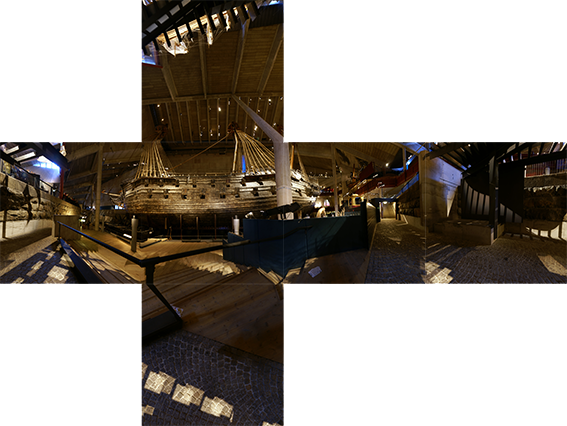
\includegraphics[height=\imageHeight]{images/cubemap.png}
		\caption{Cube mapa.}
		\label{img:cubemap}
	\end{center}
\end{figure}
\newpage
\noindent
Pre každý vrchol bubliny sa následne vypočíta vektor odrazu, pomocou ktorého sa potom vypočíta príslušný texel z cube mapy. Tento texel je následne zmiešaný s farbou bubliny a na záver je na výslednú farbu aplikovaný spomínaný alpha blending.



